
\begin{figure}[p]
	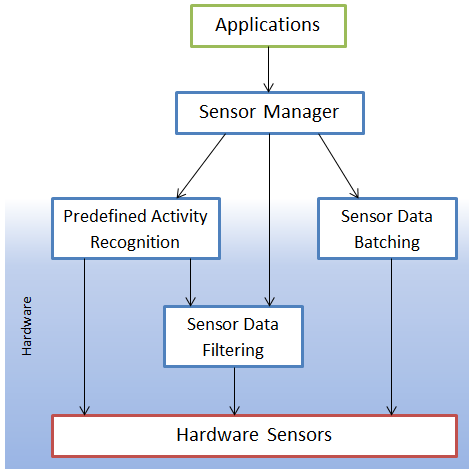
\includegraphics[width=9cm]{android_architecture_proposed.png}
	\caption{Smart sensor architecture}
    \label{fig:smartarchitecture}
\end{figure}


\section{Smart Sensors}
\label{sec:approach}

Our aim is to enable low-power, continuous sensing tasks on mobile
processors.  As described earlier, the current approaches for low
power sensing trade ease of programming with the generality of the
approach. On the one hand, fully programmable offloading of code to
low-power processors allows developing arbitrary
applications~\cite{reflex,turducken}. However, it raises several
challenges, such as requiring a split or complete redevelopment of
application functionality, and carefully choosing the code that can be
offloaded so that it can run in real time. The latter is complicated
because it depends on the type and functionality of the low-power
processor that is available.  Furthermore, since each application is
written independently, this approach makes it hard to optimize power
consumption for multiple sensing applications. Alternatively, the
phone can be designed to support a predefined set of activities but
this approach limits the number and types of applications that can be
supported.

Our approach for low-power sensing takes a middle ground and provides
a filter-based sensor API for application programs. Applications
create {\em custom wake up conditions} for events of interest by
choosing from a pre-specified set of filtering algorithms and tunning
their parameters.  When these events occur, the main processor is
woken up and the application code is invoked. The result is that
applications view the sensors as ``smart'' sensors that generate
relevant events only. This approach enables supporting a large number
of sensing applications while being significantly easier to program
compared to fully programmable offloading, as we show later. Since the
filters are pre-specified, their implementations can be optimized for
each low-power processor. Furthermore, it is possible to optimize the
operation of multiple applications that have filters in common.

Figure~\ref{fig:smartarchitecture} shows the logical architecture of a
system that implements the smart sensors abstraction.  Applications
interact with a sensor manager and define custom wake up conditions by
choosing among the avialable pre-defined filters.  The figure also
shows the that architecture supports recognition libraries that
encapsulate the functionality of the smart sensor to provide simple
wake up conditions for a large number of activities.  To keep the
complexity of filters low, our initial implementation limits filters
to operations on data collected from a single sensor.  Applications
that perform sensor fusion, are impemented by defining separate
indepedent wake up conditions on multiple sensors, and merging data on
the main processor.





The main challenge with our smart sensors approach is defining the
appropriate set of event filters for each sensor. First, the filters
need to be mainly computational tasks. Any code that needs to use
resources not available to the low-powered processor, e.g., the
graphical user interface, needs to run on the main processor. Second,
there is a trade-off in the computational tasks that are carried out
by the low-power processor. Pushing additional computation to the
low-power processor will generally result in higher accuracy filters,
and the main processor will remain asleep for longer periods of time,
thus increasing energy savings. However, this computation needs to be
performed on the low-power processor in real time, and the main
processor woken as soon as the event is detected. We evaluate this
trade-off between filter accuracy and power savings by comparing the
behavior of two different low-power processors.




We examine the types of computation performed by various sensing applications to
determine a common set of filters that are needed for these applications. In our
experience, while the application logic varies widely, their sensor event
detection algorithms are relatively simple and have commonalities. For example,
an accelerometer-based fall detector looks for acceleration that represents
free-fall, followed by a spike in acceleration~[TODO:cite]. Similarly, a step
detection algorithm looks for a local maxima within a certain range of
acceleration~[TODO:cite]. 

These applications often perform some common initial steps. For example, several
accelerometer-based applications initially check whether the acceleration
magnitude exceeds a certain threshold in order to determine if there is any
movement. Also, the acceleration data has significant noise, and hence many
applications implement low-pass filters to smoothen the accelerometer readings.
If multiple accelerometer-based applications are running at the same time, they
are each checking for these events independently, possibly resulting in
redundant computation. Common steps such as thresholding and low-pass filtering
are excellent candidates for event filters.

